% Options for packages loaded elsewhere
\PassOptionsToPackage{unicode}{hyperref}
\PassOptionsToPackage{hyphens}{url}
%
\documentclass[
]{article}
\usepackage{lmodern}
\usepackage{amssymb,amsmath}
\usepackage{ifxetex,ifluatex}
\ifnum 0\ifxetex 1\fi\ifluatex 1\fi=0 % if pdftex
  \usepackage[T1]{fontenc}
  \usepackage[utf8]{inputenc}
  \usepackage{textcomp} % provide euro and other symbols
\else % if luatex or xetex
  \usepackage{unicode-math}
  \defaultfontfeatures{Scale=MatchLowercase}
  \defaultfontfeatures[\rmfamily]{Ligatures=TeX,Scale=1}
\fi
% Use upquote if available, for straight quotes in verbatim environments
\IfFileExists{upquote.sty}{\usepackage{upquote}}{}
\IfFileExists{microtype.sty}{% use microtype if available
  \usepackage[]{microtype}
  \UseMicrotypeSet[protrusion]{basicmath} % disable protrusion for tt fonts
}{}
\makeatletter
\@ifundefined{KOMAClassName}{% if non-KOMA class
  \IfFileExists{parskip.sty}{%
    \usepackage{parskip}
  }{% else
    \setlength{\parindent}{0pt}
    \setlength{\parskip}{6pt plus 2pt minus 1pt}}
}{% if KOMA class
  \KOMAoptions{parskip=half}}
\makeatother
\usepackage{xcolor}
\IfFileExists{xurl.sty}{\usepackage{xurl}}{} % add URL line breaks if available
\IfFileExists{bookmark.sty}{\usepackage{bookmark}}{\usepackage{hyperref}}
\hypersetup{
  pdftitle={Energy Insecurity and Redlined America},
  pdfauthor={A. Justin Kirkpatrick},
  hidelinks,
  pdfcreator={LaTeX via pandoc}}
\urlstyle{same} % disable monospaced font for URLs
\usepackage[margin=1in]{geometry}
\usepackage{color}
\usepackage{fancyvrb}
\newcommand{\VerbBar}{|}
\newcommand{\VERB}{\Verb[commandchars=\\\{\}]}
\DefineVerbatimEnvironment{Highlighting}{Verbatim}{commandchars=\\\{\}}
% Add ',fontsize=\small' for more characters per line
\usepackage{framed}
\definecolor{shadecolor}{RGB}{248,248,248}
\newenvironment{Shaded}{\begin{snugshade}}{\end{snugshade}}
\newcommand{\AlertTok}[1]{\textcolor[rgb]{0.94,0.16,0.16}{#1}}
\newcommand{\AnnotationTok}[1]{\textcolor[rgb]{0.56,0.35,0.01}{\textbf{\textit{#1}}}}
\newcommand{\AttributeTok}[1]{\textcolor[rgb]{0.77,0.63,0.00}{#1}}
\newcommand{\BaseNTok}[1]{\textcolor[rgb]{0.00,0.00,0.81}{#1}}
\newcommand{\BuiltInTok}[1]{#1}
\newcommand{\CharTok}[1]{\textcolor[rgb]{0.31,0.60,0.02}{#1}}
\newcommand{\CommentTok}[1]{\textcolor[rgb]{0.56,0.35,0.01}{\textit{#1}}}
\newcommand{\CommentVarTok}[1]{\textcolor[rgb]{0.56,0.35,0.01}{\textbf{\textit{#1}}}}
\newcommand{\ConstantTok}[1]{\textcolor[rgb]{0.00,0.00,0.00}{#1}}
\newcommand{\ControlFlowTok}[1]{\textcolor[rgb]{0.13,0.29,0.53}{\textbf{#1}}}
\newcommand{\DataTypeTok}[1]{\textcolor[rgb]{0.13,0.29,0.53}{#1}}
\newcommand{\DecValTok}[1]{\textcolor[rgb]{0.00,0.00,0.81}{#1}}
\newcommand{\DocumentationTok}[1]{\textcolor[rgb]{0.56,0.35,0.01}{\textbf{\textit{#1}}}}
\newcommand{\ErrorTok}[1]{\textcolor[rgb]{0.64,0.00,0.00}{\textbf{#1}}}
\newcommand{\ExtensionTok}[1]{#1}
\newcommand{\FloatTok}[1]{\textcolor[rgb]{0.00,0.00,0.81}{#1}}
\newcommand{\FunctionTok}[1]{\textcolor[rgb]{0.00,0.00,0.00}{#1}}
\newcommand{\ImportTok}[1]{#1}
\newcommand{\InformationTok}[1]{\textcolor[rgb]{0.56,0.35,0.01}{\textbf{\textit{#1}}}}
\newcommand{\KeywordTok}[1]{\textcolor[rgb]{0.13,0.29,0.53}{\textbf{#1}}}
\newcommand{\NormalTok}[1]{#1}
\newcommand{\OperatorTok}[1]{\textcolor[rgb]{0.81,0.36,0.00}{\textbf{#1}}}
\newcommand{\OtherTok}[1]{\textcolor[rgb]{0.56,0.35,0.01}{#1}}
\newcommand{\PreprocessorTok}[1]{\textcolor[rgb]{0.56,0.35,0.01}{\textit{#1}}}
\newcommand{\RegionMarkerTok}[1]{#1}
\newcommand{\SpecialCharTok}[1]{\textcolor[rgb]{0.00,0.00,0.00}{#1}}
\newcommand{\SpecialStringTok}[1]{\textcolor[rgb]{0.31,0.60,0.02}{#1}}
\newcommand{\StringTok}[1]{\textcolor[rgb]{0.31,0.60,0.02}{#1}}
\newcommand{\VariableTok}[1]{\textcolor[rgb]{0.00,0.00,0.00}{#1}}
\newcommand{\VerbatimStringTok}[1]{\textcolor[rgb]{0.31,0.60,0.02}{#1}}
\newcommand{\WarningTok}[1]{\textcolor[rgb]{0.56,0.35,0.01}{\textbf{\textit{#1}}}}
\usepackage{graphicx,grffile}
\makeatletter
\def\maxwidth{\ifdim\Gin@nat@width>\linewidth\linewidth\else\Gin@nat@width\fi}
\def\maxheight{\ifdim\Gin@nat@height>\textheight\textheight\else\Gin@nat@height\fi}
\makeatother
% Scale images if necessary, so that they will not overflow the page
% margins by default, and it is still possible to overwrite the defaults
% using explicit options in \includegraphics[width, height, ...]{}
\setkeys{Gin}{width=\maxwidth,height=\maxheight,keepaspectratio}
% Set default figure placement to htbp
\makeatletter
\def\fps@figure{htbp}
\makeatother
\setlength{\emergencystretch}{3em} % prevent overfull lines
\providecommand{\tightlist}{%
  \setlength{\itemsep}{0pt}\setlength{\parskip}{0pt}}
\setcounter{secnumdepth}{-\maxdimen} % remove section numbering
\usepackage{bbm}
\usepackage{threeparttable}
\usepackage{float}
\usepackage{booktabs}

\title{Energy Insecurity and Redlined America}
\author{A. Justin Kirkpatrick}
\date{2021-02-05}

\begin{document}
\maketitle

\hypertarget{thanks-heartland-2017-brian-murray-and-nicinstitute}{%
\section{Thanks: Heartland 2017, Brian Murray and
NicInstitute}\label{thanks-heartland-2017-brian-murray-and-nicinstitute}}

\hypertarget{introduction}{%
\section{Introduction}\label{introduction}}

The energy insecurity literature contains evidence that low-income
households frequently face excessive energy bills, despite their income
limitations, that initially seem counter-intuitive (Hernaandez et al.,
2014; Hernaandez and Bird, 2010). Poliycmakers have expressed concern
not just that low-income households spend a larger share of income on
energy services, a measure known as \emph{energy burden}, but that
low-income households are paying more to attain the \emph{same} level of
energy services relative to other income groups. The notion of inequity
in energy access - the ability to purchase energy services such as home
heating or cooling - has been the object of programs that aim to improve
residential energy efficiency through retrofits (CITE), or provide
subsidies for newer, higher-efficiency appliances (CITE). As part of
increasing concerns about income inequality, energy burden has become a
notable issue.

Some of this insecurity is attributable to the housing stock, which is
less energy effcient in low income and minority neighborhoods. Previous
work in this area has found negative correlations between energy
efficiency and racial characteristics at the census block-group level
(Reames, 2016b), and many have noted the disproportionate energy burden
faced by low-income households. With tight budget constraints,
low-income households are more likely to consume lower-priced housing.
Naturally, lower priced housing stock will be deficient in some areas.
Maintenance may be less frequent or non-existent, structural problems
may plague the home, and the home may have un-remediated lead paint or
asbestos. Similarly, it is more likely that the home is poorly
insulated, has single-pane windows, and has dated, inefficient systems
for heating and cooling. These characteristics are common amongst
low-income housing, and are intertwined with poor child health and
development outcomes, and with food insecurity (Cook et al., 2008).

That a high energy burden is common amongst low-income households and
those who face food insecurity is not surprising as energy burden is, by
definition, decreasing in income. However, even when controlling for
poverty rates, Reames (2016b) finds that minority-dominated census
block-groups and those block-groups with high measures of racial
segregation also tend to have lower (worse) energy efficiency. That is,
even conditional on poverty, minority areas may have lower-efficiency
housing stock relative to non-minority areas. Not only is energy
insecurity an issue, but so too is energy inequity, which I define as
``the disproportional incidence of energy insecurity in heavily-minority
areas relative to non-minority areas of similar income.''

This brings about the questions central to this paper: First, is there
evidence that racial differences in energy burden exist once income and
wealth are accounted for? Second, what drives the wedge between the
energy efficiency of the housing stock available to (or chosen by)
minorities and the energy efficiency of the housing stock available to
(or chosen by) non-minorities of similar economic status?

This paper posits a hypothesis for one potential cause of this wedge and
why it persists over time. I propose that institutional discrimination
in the 1930s-1970s forced African-Americans and other minorities into
segregated ``redlined'' communities and, over this period, the housing
stock in these communities, though similar at one point in time,
developed differently relative to the housing stock of non-redlined
communities of similar socio-economic standing and demographic
composition. This historical racism has persistent long-term effects on
housing choices and housing quality that explains, at least in part, the
energy inequity we observe today.

To this end, I explore the extent to which minority households face
energy inequity - that is, the extent to which minority households pay a
higher amount for the same level of energy services such as home heating
relative to non-minorities of similar socio-economic status. I do this
by examining data on home energy consumption, race, and income. This
requires careful attention to the nature of energy expenditures. High
levels of energy expenditure may be a sign that a household values warm
temperatures during Winter months and chooses to spend a larger share of
income on home heating. High levels of energy expenditure may also be
the result of households who choose a home with very low energy
efficiency and who must spend a great deal simply to keep the interior
temperature at a low but livable temperature. In short, one can spend a
lot of money to heat to 75 degrees farenheit in an efficient home, and
one can spend a lot of money heating to 60 degrees farenheit in a very
inefficient home. The two are observationally equivalent when examining
only monthly bills and outside temperature. I disentangle these two by
leveraging data from the California Residential Appliance Saturation
Survey (RASS) which includes consumer's reported thermostat setpoint,
combined with a simple model of household energy consumption. The model
allows me to separate unobserved characteristics of the household from
home heating efficiency, permitting unbiased estimation of a household's
home heating response to cold-weather shocks. By focusing on the energy
consumption response after controlling for the household's thermostat
setpoint, I am able to measure the home's energy efficiency level,
rather than the household's preference for indoor temperatures.

Using original maps from the Homeowners Loan Corporation (HOLC) which
designated ``redlined'' areas along with ``yellow'', ``green'' and
``blue'' areas in more than 170 cities in the US in 1933-36
\ref{fig:HOLC1}, combined with RASS survey data from 2009, I test the
hypothesis that areas designated Grade D (or ``red''), which were
considered ``appropriate'' for minorities to purchase homes, have more
frequent substandard heating systems and are more inefficient in
heating, evidenced by higher cost responses to cold weather shocks after
controlling for thermostat setpoints. As noted by (CITE SPENCER), the
HOLC maps did not randomly assign neighborhoods grades and therefore any
current differences in the simple mean of energy efficiency outcomes
between areas of different grades should not be causally attributed to
redlining policy. Specifically, areas of lower construction quality,
lower rent, older and smaller homes, and areas with pre-existing
minority populations in 1933-36 were more likely to be graded as
``red.'' To address the potential for bias, I control for these
observables by using original survey data recorded by HOLC surveyors in
1933-36 that recorded the justification for grading. Notably, there is
considerable overlap in rents, the presence of minority populations,
income, and other observables between ``red'' and ``yellow'' HOLC
grades, leaving specific designation by the surveyor to be nearly
random. Conditional on these observables and assuming that unobserved
differences correlated with HOLC grade do not still apply in the current
period, then ``red'' grades are as good as randomly assigned. I use this
conditionally as-good-as-random assignment to estimate causal effects of
HOLC ``redlining'' on current energy inefficiency and energy inequity.

\begin{center}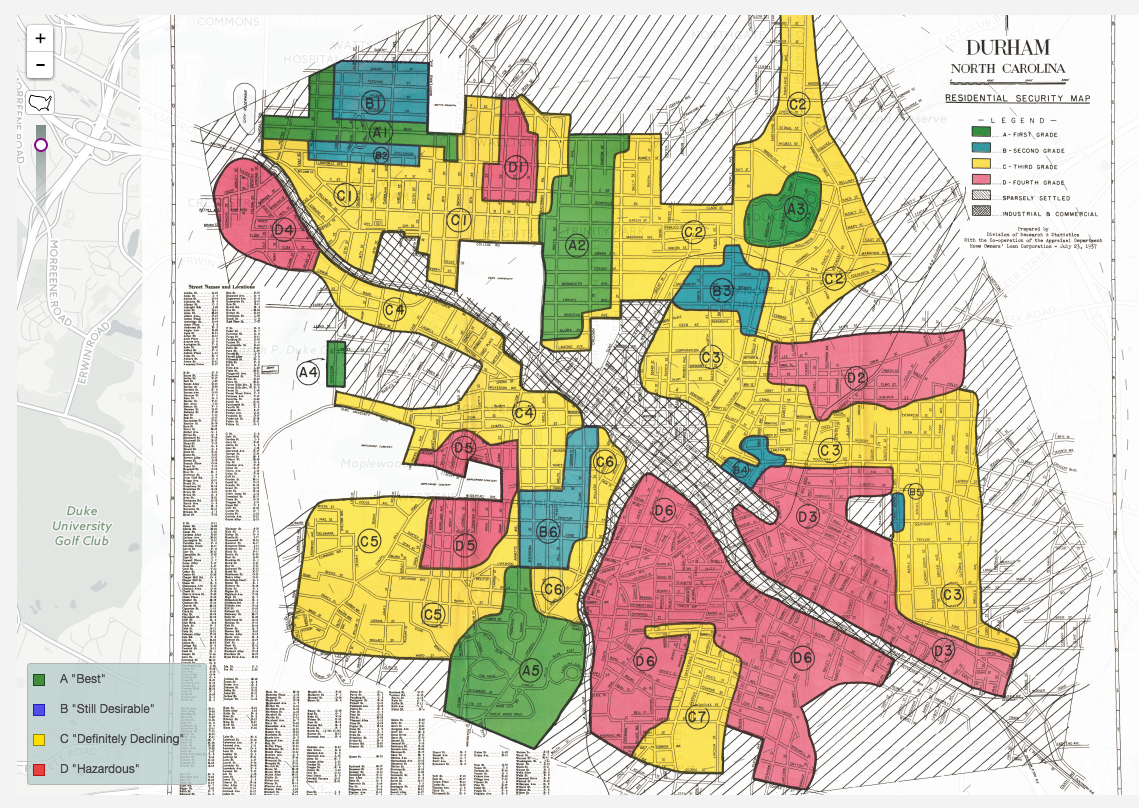
\includegraphics[width=0.9\linewidth]{D:/user/ajk41/Low Income Energy/Images/HOLC_example_1} \end{center}

This paper does not address the dynamics of residential sorting between
1933 and the current period. While the practice of ``redlining'' came to
a statutory end with the Civil Rights Act of 1968, it was not until
1977's Community Reinvestment Act that lenders were required to detail
the extent of their lending in all areas in which they operated,
including in heavily-minority ``redlined'' neighborhoods. \emph{De
facto}, rather than \emph{de jure} housing discrimination continued well
beyond that date, and still continues today, albeit in different ways
(see Christensen + Timmins, \ldots). In a housing market with no
frictions and no discrimination, post-institutional redlining would have
seen a re-sorting of households by preferences for housing stock. In
this perfect case, observed differences in energy inequity would be the
result of households sorting in to inefficient units, and housing prices
adjusting to reflect the cost of heating. In effect, the most
inefficient units would be rented by those who have little preference
for warm tempertures. At the same time, poverty is known to be cyclic,
and low-income populations that rely heavily on family and community may
have, in effect, high fixed costs of moving outside of a neighborhood.
For young families especially, remaining close to (grand)parents may
necessitate remaining in the same neighborhood for multiple generations.
To the extent that a policy in place through 1979 ``fixed'' a family's
location by precluding moves to other areas with better housing stock,
the same families may face high costs of moving today. Thus, redlining
policy may have a \emph{hysteresis} effect today. A full sorting model
of residential choice is beyond this paper, though not infeasible under
the right data circumstances.

This paper contributes to two separate literatures. The first literature
is the body of work that examines the role of historic discriminatory
economic policies on current outcomes. In this area, this paper is most
similar to Aaronson and Mazumder (???), which specifically examines the
effect of HOLC redlining on credit and home ownership, Aaronson and
Mazumder use a boundary difference-in-differences to show that
households located inside HOLC redlined areas had less access to credit
and were less likely to own their home relative to similar households
located just outside the boundary. That striking result motivates this
paper -- one of the mechanisms by which energy inequity can manifest is
through declining investment in available housing stock either by
owner-occupants or by absentee landlords. Energy inequity is, at least
in theory, a direct result of the effect shown by Aaronson and Mazumder.
The second literature examines household electricity consumption
responses to temperature or price shocks in the context of energy
expenditures. Largely motivated by the need to accurately predict future
electricity consumption under future prices, demographics, or climate
(Ang. and Auffhamer 2009), these studies have examined the consumption
response to varying temperature or prices. Few, however, have
incorporated a model of consumption that allows for endogenous
preferences for thermostat setpoints. An exception is Brewer (2019), who
estimates a ``bliss point'' in a structural model of joint residence and
thermostat setpoint choice, though this paper examines moral hazard in
landlord-paid heating. The paper most similar to this is Doremus, Jacqz,
and Johnston (2020), who examine household energy consumption
expenditures in response to variation in temperature by income. However,
the authors similarly do not allow for endogenous thermostat setpoints
that reflect unobserved tastes.

Section 2 defines energy inequity and introduces a simple model of home
heating costs. It further shows how unobserved home efficiency
characteristics, which may vary between redlined and non-redlined
neighborhoods when historic housing discrimination still impacts current
energy burdens,\\
can be estimated from energy consmption data with a known thermostat
setpoint. Section 3 introduces the data. Section 4 discusses the
estimation strategy. Section 5 presents results and Section 6 concludes.

Some citations: Aroonreuengsawat and Auffhammer: reponse to weather
shocks, but does not endogenize the thermostat setpoint Levinson 2013
(JEBO) on building codes: not using thermostats, just decomposing
aggregate (state, region) decrease in PerCap energy by demos, moving,
buildings, etc. Does use RECS, but only to get CA and NON-CA HDD
responses (no thermostat) Chong 2013: estimates response but no
thermostat \#\# Details and description

\hypertarget{energy-inequity-and-housing-discrimination}{%
\section{2. Energy Inequity and Housing
Discrimination}\label{energy-inequity-and-housing-discrimination}}

\hypertarget{define-energy-burden.}{%
\paragraph{Define energy burden.}\label{define-energy-burden.}}

Energy burden is defined as the share of total household income spent on
energy purchases not including transport. The low-income energy burden
is the noted phenomenon where low-income households have a
disproportionate likelihood of having a high proportion of household
income devoted to energy purchases (Byrne 1986; Baxter 1998). In
practice, energy burdens above 10\% are worrisome, and many households
have burdens of 20\% or more (Baxter, 1988). Middle and upper-income
households tend to spend 5\% or less of household income on energy
services (Hernandez and Bird, 2010). High energy burden indicates an
inability to afford basic energy services (heating, refrigeration),
particularly during periods of volatility in energy prices.

\hypertarget{cite-severity-of-problem}{%
\paragraph{Cite severity of problem}\label{cite-severity-of-problem}}

\hypertarget{link-between-energy-burden-and-energy-efficiency}{%
\paragraph{Link between energy burden and energy
efficiency}\label{link-between-energy-burden-and-energy-efficiency}}

\hypertarget{obvious-reason-being-poor-and-short-sighted}{%
\paragraph{Obvious reason: being poor and
short-sighted}\label{obvious-reason-being-poor-and-short-sighted}}

\hypertarget{conditional-on-income-problem-still-persists}{%
\paragraph{Conditional on income, problem still
persists!}\label{conditional-on-income-problem-still-persists}}

\hypertarget{potential-explanations-brief}{%
\paragraph{Potential explanations
(brief)}\label{potential-explanations-brief}}

This section is brief. Full literature review comes later. Or maybe the
full lit for why is here?

\hypertarget{causal-chain-is-really-long}{%
\paragraph{Causal chain is really
long}\label{causal-chain-is-really-long}}

\hypertarget{potential-chain-redlining-lack-of-ownership-why-stay-in-area}{%
\paragraph{Potential chain (redlining--\textgreater{} lack of ownership
--\textgreater{} why stay in
area?)}\label{potential-chain-redlining-lack-of-ownership-why-stay-in-area}}

\hypertarget{this-paper-here}{%
\subsection{This paper here\ldots{}}\label{this-paper-here}}

\hypertarget{explores-the-role-of-redlining-in-explaining-energy-burden}{%
\paragraph{Explores the role of redlining in explaining energy
burden}\label{explores-the-role-of-redlining-in-explaining-energy-burden}}

By isolating the energy outcomes that can only be explained by redlining

\hypertarget{plausibly-exogenous-variation}{%
\paragraph{Plausibly exogenous
variation}\label{plausibly-exogenous-variation}}

Conditional on similar (but not red-lined) nearby neighborhoods.
Observables.

\hypertarget{extracted-1930s-data-to-understand-redlining}{%
\paragraph{Extracted 1930's data to understand
redlining}\label{extracted-1930s-data-to-understand-redlining}}

Survey data created by federal HOLC employees in 1936-1939 provides
neighborhood-specific data on observable characteristics that can be
used to identify the effects of redlining. The designation of red- and
yellow-lined areas (as well as green and blue) aggregate away important
variation between each grading. Not all redlined areas are identical,
nor are all yellow areas. Survey data recorded as part of the redline
designation process provides important, but largely unusued, sources of
variation. Within-grade variation in housing is common with reported
average rents, median income, repair status of housing, share of housing
developed, and construction type. Prior to being redlined, areas with
high percentages of low-income or minority populations were more likely
to have lower rents and lower housing quality. Frequently, the reason
for a low-income or minority area's location was associated with the
quality of the geography or proximity to natural features - low-lying
areas that frequently flooded or areas too steep for conventional
building were generally populated by lower-income individuals. These
same features also foment low investment in housing stock, and can
explain current inefficiencies in housing regardless of the HOLC grade.
With HOLC survey data in hand, I can control for these features and
separate out the effect of HOLC redlining from the determinants of HOLC
grading.

\hypertarget{identification-key-there-are-neighborhoods-with-identical-economics-and-racial-composition-where-some-surveyors-designated-them-red-and-some-designated-yellow.}{%
\paragraph{Identification key: there are neighborhoods with identical
economics and racial composition where some surveyors designated them
red and some designated
yellow.}\label{identification-key-there-are-neighborhoods-with-identical-economics-and-racial-composition-where-some-surveyors-designated-them-red-and-some-designated-yellow.}}

\hypertarget{poor-whites-vs.-poor-blacks}{%
\paragraph{Poor whites vs.~poor
blacks}\label{poor-whites-vs.-poor-blacks}}

\hypertarget{historic-data-merged-to-block-groups-to-leverage-modern-outcomes}{%
\paragraph{Historic data merged to block groups to leverage modern
outcomes}\label{historic-data-merged-to-block-groups-to-leverage-modern-outcomes}}

To assess current energy outcomes, I merge original HOLC neighborhoods
to modern census block groups, extracting ACS and census indicators of
high energy burden. Census block groups match the granularity of HOLC
neighborhoods reasonably well. However, boundaries do not tend to
coincide exactly, requiring some aggregation. Once linked, I compare
modern energy outcomes with HOLC grading, conditioning on observable
characteristics both in the 1930's (selection), and in the present.
While an individual household-level analysis would provide the clearest
evidence, household-level energy consumption data is limited for privacy
reasons, especially at the spatial resolution of HOLC neighborhoods,
which can have as few as 100 homes in them.

\hypertarget{section}{%
\paragraph{}\label{section}}

\hypertarget{data}{%
\section{Data}\label{data}}

This is the section with the data. And the section where we process the
data

\hypertarget{census-blockgroups}{%
\subsection{Census blockgroups}\label{census-blockgroups}}

\newpage

\hypertarget{substandard-heating-fuel-by-holc-grade}{%
\subsubsection{Substandard heating fuel by HOLC
grade}\label{substandard-heating-fuel-by-holc-grade}}

\begin{table}

\caption{\label{tab:substandard-est-2}Share of Households with OtherSubstandardNarrow Fuel (Coal and none) by HOLC Grade\label{tab:substandardnarrow1}}
\centering
\resizebox{\linewidth}{!}{
\begin{tabular}[t]{lcccccccc}
\toprule
  & Model 1 & Model 2 & Model 3 & Model 4 & Model 5 & Model 6 & Model 7 & Model 8\\
\midrule
as.factor(GRADE.max)D & 0.00348** & 0.00338** & 0.00477** & 0.00383** & 0.00441*** & 0.00533*** & 0.00263 & 0.00515*\\
 & (0.00158) & (0.00159) & (0.00189) & (0.00155) & (0.00122) & (0.00181) & (0.00176) & (0.00302)\\
as.factor(GRADE.max)B & -0.00040 & -0.00032 & -0.00062 & -0.00031 & 0.00039 & -0.00066 & 0.00303 & 0.00777\\
 & (0.00112) & (0.00120) & (0.00147) & (0.00099) & (0.00146) & (0.00121) & (0.00385) & (0.01007)\\
as.factor(GRADE.max)A & 0.00025 & -0.00053 & -0.00571 & -0.00075 & -0.00004 & -0.00594 & -0.00414 & -0.02233\\
 & (0.00343) & (0.00338) & (0.00510) & (0.00332) & (0.00365) & (0.00504) & (0.00890) & (0.01409)\\
MedIncome2018 & -0.00009*** & -0.00010*** & -0.00011*** & -0.00012*** & -0.00012*** & -0.00013*** & -0.00017*** & -0.00023***\\
 & (0.00002) & (0.00002) & (0.00002) & (0.00002) & (0.00002) & (0.00002) & (0.00003) & (0.00005)\\
MedIncome1936 & 0.00026** & 0.00003 & 0.00006 & 0.00009 & 0.00007 & 0.00012 & -0.00014 & -0.00024\\
 & (0.00011) & (0.00014) & (0.00014) & (0.00014) & (0.00015) & (0.00015) & (0.00066) & (0.00107)\\
Rent3739\_Mean & 0.00007* & 0.00007* & 0.00005 & 0.00006* & 0.00006* & 0.00005 & 0.00003 & 0.00005\\
 & (0.00004) & (0.00003) & (0.00005) & (0.00003) & (0.00003) & (0.00005) & (0.00002) & (0.00005)\\
MedIncome2018 × MedIncome1936 &  & 0.00000** & 0.00000*** & 0.00000*** & 0.00000** & 0.00000** & 0.00001 & 0.00003\\
 &  & (0.00000) & (0.00000) & (0.00000) & (0.00000) & (0.00000) & (0.00001) & (0.00002)\\
Black &  &  &  & -0.00219 & -0.00115 & -0.00104 & -0.00541 & -0.00688\\
 &  &  &  & (0.00455) & (0.00577) & (0.00481) & (0.00930) & (0.01490)\\
White &  &  &  & 0.00304 & 0.00303 & 0.00464 & 0.00648 & 0.00890\\
 &  &  &  & (0.00436) & (0.00454) & (0.00527) & (0.00805) & (0.01295)\\
Asian &  &  &  & -0.00011 & 0.00001 & 0.00108 & -0.00326 & -0.00356\\
 &  &  &  & (0.00451) & (0.00490) & (0.00523) & (0.01133) & (0.01692)\\
as.factor(GRADE.max)D × Black &  &  &  &  & -0.00199 &  &  & \\
 &  &  &  &  & (0.00411) &  &  & \\
as.factor(GRADE.max)B × Black &  &  &  &  & -0.00285 &  &  & \\
 &  &  &  &  & (0.00273) &  &  & \\
as.factor(GRADE.max)A × Black &  &  &  &  & -0.00573 &  &  & \\
 &  &  &  &  & (0.01121) &  &  & \\
NBlack\_YN &  &  &  &  &  &  & -0.00211 & 0.00131\\
 &  &  &  &  &  &  & (0.00316) & (0.00371)\\
NBlack\_PCT &  &  &  &  &  &  & -0.00000 & -0.00002\\
 &  &  &  &  &  &  & (0.00004) & (0.00005)\\
\midrule
Num.Obs. & 4629 & 4629 & 3313 & 4629 & 4629 & 3313 & 1034 & 690\\
R2 & 0.097 & 0.098 & 0.097 & 0.101 & 0.101 & 0.100 & 0.100 & 0.111\\
R2 Adj. & 0.086 & 0.087 & 0.081 & 0.089 & 0.089 & 0.084 & 0.052 & 0.049\\
R2 Within & 0.021 & 0.021 & 0.026 & 0.025 & 0.025 & 0.030 & 0.032 & 0.044\\
R2 Pseudo &  &  &  &  &  &  &  & \\
AIC & -22109.1 & -22110.3 & -15583.4 & -22120.6 & -22115.8 & -15590.5 & -4692.8 & -3006.6\\
BIC & -21742.0 & -21736.8 & -15235.4 & -21727.7 & -21703.7 & -15224.2 & -4426.0 & -2797.9\\
Log.Lik. & 11111.557 & 11113.148 & 7848.704 & 11121.281 & 11121.917 & 7855.252 & 2400.393 & 1549.309\\
FE: STCO & X & X & X & X & X & X & X & X\\
Std. errors & Clustered (STCO) & Clustered (STCO) & Clustered (STCO) & Clustered (STCO) & Clustered (STCO) & Clustered (STCO) & Clustered (STCO) & Clustered (STCO)\\
HOLC Grade Threshold & 80\% & 80\% & 95\% & 80\% & 80\% & 95\% & 80\% & 95\%\\
\bottomrule
\multicolumn{9}{l}{\textsuperscript{} * p < 0.1, ** p < 0.05, *** p < 0.01}\\
\multicolumn{9}{l}{\textsuperscript{} Robust SE clustered by FIPS county}\\
\multicolumn{9}{l}{\textsuperscript{} Columns 1, 2, 3, 5 are blokgroups with >80\% of total area in one HOLC grade; 4, 6, and 8 are >95\%}\\
\end{tabular}}
\end{table}

\hypertarget{results}{%
\paragraph{Results}\label{results}}

Column 1 allows an additive effect for median income in 2018 and 1936
(reported from HOLC surveys), while 2-8 allow an interaction.

As expected, current median blockgroup income predicts a lower share of
homes with substandard heating fuel across all models. Median income in
1936 predicts \textbf{higher} prevalance of substandard heating in
higher 1936 median income areas.

Columns 4-7 include controls for current racial composition. These
results consistently find that higher percentages of Blacks are
associated with lower likelihood of substandard heating fuel.
\textbf{EXPLAIN!!}

The coefficient on HOLC Grade D is positive and significant across
almost all specifications, indicating that, conditional on a rich set of
controls including 1936 characteristics to control for selection on
observables, areas that were graded ``D'' by the HOLC are more likely to
have substandard heating fuels in 2018 relative to those graded ``C''.

\begin{table}

\caption{\label{tab:substandard-est-3}Share of Households with OtherSubstandardWide Fuel (Coal + Wood + OtherFuel + LPGas + FuelOil + NoFuel) by HOLC Grade}
\centering
\resizebox{\linewidth}{!}{
\begin{tabular}[t]{lcccccccc}
\toprule
  & Model 1 & Model 2 & Model 3 & Model 4 & Model 5 & Model 6 & Model 7 & Model 8\\
\midrule
as.factor(GRADE.max)D & -0.01152 & -0.01222 & -0.01204 & -0.00967 & -0.00546 & -0.00883 & -0.00200 & 0.01353\\
 & (0.00850) & (0.00832) & (0.01079) & (0.00892) & (0.01440) & (0.01138) & (0.00645) & (0.01363)\\
as.factor(GRADE.max)B & 0.01167 & 0.01221 & 0.00820 & 0.01289 & 0.01637 & 0.00828 & 0.02788* & 0.01265\\
 & (0.01199) & (0.01269) & (0.01367) & (0.01081) & (0.01263) & (0.01118) & (0.01594) & (0.02766)\\
as.factor(GRADE.max)A & -0.00161 & -0.00708 & -0.00375 & -0.00884 & -0.00559 & -0.00521 & 0.02525 & 0.02926\\
 & (0.02184) & (0.02226) & (0.03052) & (0.02138) & (0.02320) & (0.02852) & (0.04053) & (0.07853)\\
MedIncome2018 & -0.00019 & -0.00027 & -0.00029 & -0.00040* & -0.00041 & -0.00044 & 0.00004 & 0.00042**\\
 & (0.00031) & (0.00034) & (0.00039) & (0.00024) & (0.00025) & (0.00027) & (0.00017) & (0.00020)\\
MedIncome1936 & 0.00199*** & 0.00038 & -0.00008 & 0.00118 & 0.00105 & 0.00093 & 0.00013 & 0.02053***\\
 & (0.00061) & (0.00079) & (0.00091) & (0.00088) & (0.00085) & (0.00086) & (0.00319) & (0.00678)\\
Rent3739\_Mean & 0.00031 & 0.00031 & 0.00032 & 0.00028 & 0.00028 & 0.00027 & 0.00002 & 0.00005\\
 & (0.00023) & (0.00023) & (0.00029) & (0.00020) & (0.00020) & (0.00023) & (0.00005) & (0.00011)\\
MedIncome2018 × MedIncome1936 &  & 0.00002* & 0.00003* & 0.00002** & 0.00002** & 0.00003** & 0.00001 & -0.00014***\\
 &  & (0.00001) & (0.00002) & (0.00001) & (0.00001) & (0.00001) & (0.00003) & (0.00004)\\
Black &  &  &  & -0.09896 & -0.09236 & -0.11147 & 0.00215 & -0.00989\\
 &  &  &  & (0.08187) & (0.07818) & (0.08743) & (0.04618) & (0.04469)\\
White &  &  &  & -0.03509 & -0.03480 & -0.03623 & 0.04190 & 0.03795\\
 &  &  &  & (0.08027) & (0.07993) & (0.08269) & (0.04538) & (0.05130)\\
Asian &  &  &  & -0.09414 & -0.09292 & -0.10593 & -0.01257 & -0.03457\\
 &  &  &  & (0.08744) & (0.08678) & (0.09355) & (0.03699) & (0.04002)\\
as.factor(GRADE.max)D × Black &  &  &  &  & -0.01384 &  &  & \\
 &  &  &  &  & (0.02224) &  &  & \\
as.factor(GRADE.max)B × Black &  &  &  &  & -0.01385 &  &  & \\
 &  &  &  &  & (0.01474) &  &  & \\
as.factor(GRADE.max)A × Black &  &  &  &  & -0.01975 &  &  & \\
 &  &  &  &  & (0.03346) &  &  & \\
NBlack\_YN &  &  &  &  &  &  & 0.00114 & -0.00432\\
 &  &  &  &  &  &  & (0.01844) & (0.03390)\\
NBlack\_PCT &  &  &  &  &  &  & -0.00026 & -0.00036\\
 &  &  &  &  &  &  & (0.00028) & (0.00037)\\
\midrule
Num.Obs. & 4629 & 4629 & 3313 & 4629 & 4629 & 3313 & 1034 & 690\\
R2 & 0.552 & 0.553 & 0.554 & 0.569 & 0.570 & 0.575 & 0.485 & 0.447\\
R2 Adj. & 0.547 & 0.548 & 0.546 & 0.564 & 0.564 & 0.567 & 0.457 & 0.408\\
R2 Within & 0.025 & 0.027 & 0.024 & 0.062 & 0.063 & 0.071 & 0.032 & 0.052\\
R2 Pseudo &  &  &  &  &  &  &  & \\
AIC & -8311.9 & -8317.7 & -5684.2 & -8483.9 & -8480.1 & -5841.1 & -2067.2 & -1299.8\\
BIC & -7944.8 & -7944.2 & -5336.2 & -8091.0 & -8067.9 & -5474.8 & -1800.3 & -1091.1\\
Log.Lik. & 4212.958 & 4216.870 & 2899.097 & 4302.945 & 4304.035 & 2980.559 & 1087.578 & 695.913\\
FE: STCO & X & X & X & X & X & X & X & X\\
Std. errors & Clustered (STCO) & Clustered (STCO) & Clustered (STCO) & Clustered (STCO) & Clustered (STCO) & Clustered (STCO) & Clustered (STCO) & Clustered (STCO)\\
HOLC Grade Threshold & 80\% & 80\% & 95\% & 80\% & 80\% & 95\% & 80\% & 95\%\\
\bottomrule
\multicolumn{9}{l}{\textsuperscript{} * p < 0.1, ** p < 0.05, *** p < 0.01}\\
\multicolumn{9}{l}{\textsuperscript{} Robust SE clustered by FIPS county}\\
\multicolumn{9}{l}{\textsuperscript{} Columns 1, 2, 3, 5 are blokgroups with >80\% of total area in one HOLC grade; 4, 6, and 8 are >95\%}\\
\end{tabular}}
\end{table}

\hypertarget{results-1}{%
\paragraph{Results}\label{results-1}}

The same phenomenon is not observed when defining substandard heating as
including LP gas and fuel oil. In many parts of the country, LP gas and
fuel oil are commonplace, and can be relatively efficient and desirable.
It is not wholly unexpected for this to be insignificant.

\hypertarget{results-using-zip-code-tabulation-area-zcta}{%
\paragraph{Results using Zip Code Tabulation Area
(ZCTA)}\label{results-using-zip-code-tabulation-area-zcta}}

Zipcode Tabulation Areas are coarser than census blockgroups. Due to
this, there are fewer ZCTAs that fall predominantly in one HOLC grade,
resulting in a smaller sample size. Of the 2,842 zip codes that touch on
one or more HOLC neighborhoods, 45 zip codes have greater than 80\%
within one HOLC grade. Of these, 19 are Grade D (red). Of these, only 2
zip code(s) have HOLC survey data including median income, presence of
minorities, and rent data for 1936-38. This precludes the use of zip
code aggregations to estimate HOLC grading on current substandard
heating fuel.

\hypertarget{household-level-energy-consumption-ca-rass}{%
\subsection{Household-level energy consumption
(CA-RASS)}\label{household-level-energy-consumption-ca-rass}}

Aggregation can mask important heterogeneity in household energy
consumption. We use household-level monthly consumption data geolocated
to the zip-code level to identify HOLC-zone specific energy consumption
responses to cooling and heating events.

Household energy consumption data is retrieved from the California
Residential Appliance Saturation Survey (RASS) for 2009 and (hopefully)
2019. The RASS is commissioned by the California Public Utilities
Commission and implemented by DNV GL Energy Insights. The survey
contains information on household energy consumption including home age,
primary heating fuel source, and thermostat setpoint. The survey also
includes the household's zip code, household characteristics including
income and number of children, and merges two years of billing
information obtained direclty from the gas and electric utilities
serving the household. The survey sample consists of 25721 households
sampled from all over California.

We are interested in household's energy consumption response to
increases in heating degree days. We focus on households that rely
primarily on electric heating. For each household, we estimate a
consumption response function that summarizes the household's change in
electricity consumption per change in monthly heating degree days. This
measure will be larger if a household consumes more energy when
temperatures are lower, and smaller if a household consumes less energy
when temperatures drop. I allow this response to vary bsed on the HOLC
grade that covers the plurality of the zip code in which the household
lies. I use only those zip codes in which greater than 80\% of the zip
code is within one specific HOLC grade.

\emph{A priori}, it is not clear whether the interaction of heating
degree days and HOLC-designated redlining should be positive or
negative. If a household prefers to remain warm and comfortable on a
cold night, then expenditures will be higher when temperatures are
lower. Similarly, if a household in a redlined area maintains the same
indoor temperature setpoint but has a home with lower energy ratings or
is otherwise less efficient, then energy expenditures will be greater as
well. If expenditures are not greater, then it may be that the household
trades off comfort by lowering the indoor temperature in order to keep
expenditures low, or it may be that the home is very efficient, and more
energy is not needed to maintain a constant temperature. This ambiguity
confounds interpretation of estimates.

Table (below) reports the results from a regression of the form:

\[hdd^e_h = \beta_0 + \sum 1(grade_h=g)\beta_g + \beta_{inc} avgincome_h + cdd^e_h + \gamma^{CZ} + \varepsilon\]

Where \(hdd^e\) is the electricity consumption response to one
additional heating degree day for household \(h\) located in HOLC grade
\(g\). \(cdd^e\) is the household's electricity consumption response to
an additional cooling degree day. Table (below that) shows results for
\(hdd^g\). \(\gamma^{CZ}\) are climate-zone fixed effects.

\begin{table}

\caption{\label{tab:RASS-1ex}Regression of heating-degree day gas consumption response on HOLC grade and income\label{tab:responsegas1}}
\centering
\begin{tabular}[t]{lcc}
\toprule
  & Model 1 & Model 2\\
\midrule
GRADE.maxD & 0.063** & 0.063**\\
 & (0.027) & (0.027)\\
GRADE.maxC & -0.227*** & -0.227***\\
 & (0.029) & (0.029)\\
avginc & 0.000 & 0.000\\
 & (0.000) & (0.000)\\
\midrule
Num.Obs. & 14822 & 14822\\
R2 & 0.107 & 0.107\\
R2 Adj. & 0.107 & 0.107\\
R2 Within & 0.004 & 0.004\\
R2 Pseudo &  & \\
AIC & 13135.9 & 13135.9\\
BIC & 13227.2 & 13227.2\\
Log.Lik. & -6555.968 & -6555.968\\
FE: CZT24 & X & X\\
Std. errors & Clustered (CZT24) & Clustered (CZT24)\\
\bottomrule
\multicolumn{3}{l}{\textsuperscript{} * p < 0.1, ** p < 0.05, *** p < 0.01}\\
\multicolumn{3}{l}{\textsuperscript{} Using only households with gas as primary heating fuel}\\
\multicolumn{3}{l}{\textsuperscript{} Omitted grade is refactored to be "X"}\\
\end{tabular}
\end{table}

\begin{table}

\caption{\label{tab:RASS-1ex}Regression of heating-degree day electricity consumption response on HOLC grade and income\label{tab:responseelectric1}}
\centering
\begin{tabular}[t]{lcc}
\toprule
  & Model 1 & Model 2\\
\midrule
as.factor(GRADE.max)D & 1.524 & 2.738\\
 & (2.189) & (3.038)\\
avginc & 0.000 & 0.000\\
 & (0.000) & (0.000)\\
cdd.e &  & 0.946***\\
 &  & (0.232)\\
\midrule
Num.Obs. & 2239 & 2239\\
R2 & 0.139 & 0.201\\
R2 Adj. & 0.135 & 0.197\\
R2 Within & 0.029 & 0.098\\
R2 Pseudo &  & \\
AIC & 17904.3 & 17740.2\\
BIC & 17967.2 & 17808.7\\
Log.Lik. & -8941.161 & -8858.087\\
FE: CZT24 & X & X\\
Std. errors & Clustered (CZT24) & Clustered (CZT24)\\
\bottomrule
\multicolumn{3}{l}{\textsuperscript{} * p < 0.1, ** p < 0.05, *** p < 0.01}\\
\multicolumn{3}{l}{\textsuperscript{} Using only households with electricity as primary heating}\\
\multicolumn{3}{l}{fuel}\\
\multicolumn{3}{l}{\textsuperscript{} Omitted grade is actually "X" as all "C" is lost in gas}\\
\end{tabular}
\end{table}

Coefficient results in \ref{tab:responsegas1}, Model (1) indicate that
households located inside the HOLC Grade D (red) areas have
significantly higher gas responses relative to those in HOLC ungraded
areas within the urban boundary and relative to those in HOLC Grade C.
The omitted factor in \ref{tab:responsegas1} is ungraded so that results
on Grade D can be compared directly to \ref{tab:responseelectric1},
which has insufficient data to compare to Grade C.

Table \ref{tab:responseelectric1} shows significantly lower electricity
responses. In each case, only households that report primary heating
fuel of gas (first table) and electricity (second table) are included.
The ambiguity in effect is clear in examining Table
\ref{tab:responseelectric1}, which shows a significantly \emph{lower}
effect within the HOLC red (D) areas. In Grade D (red) areas, households
using natural gas for their primary heating fuel tend to have lower
response to heating degree days relative to those in Grade C.

Lower response to heating degree days can be generated by two competing
explanations. First, households in Grade D areas may have more efficient
homes and heating systems. With a sealed building envelope and modern
gas heaters, the cost to maintain the temperature inside may be low
relative to areas with drafty windows and older heating systems. A
competing explanation is that Grade D areas are far less efficient,
heating is more expensive on the margin, and households in these less
efficient homes compensate by lowering the thermostat setpoint. A home
set at 55 degrees overnight will consume less energy than a home set at
75 degrees, even if it is less efficient.

To address this confounding, I leverage the household's response to the
RASS survey question on thermostat setpoint and build a\\
model of household energy consumption.

\hypertarget{a-model-of-heating-energy-consumption}{%
\subsubsection{A model of heating energy
consumption}\label{a-model-of-heating-energy-consumption}}

Let heating energy consumed be determined by \(H(\tau_i, T_i; \phi_i)\),
where \(\tau_i\) is the household's thermostat setpoint, \(T_i\) is the
outside ambient temperature around household \(i\), and \(\phi_i\) is a
parameter summarizing the envelope and appliance efficiency of household
\(i\). Households with more efficient insulation, dual-pane windows, and
higher energy star rated heating systems will have a lower value of
\(\phi_i\). In a simple linear form, the cost of heating a home with
setpoint \(\tau_i\) in month \(J\) is:

\begin{eqnarray}
H = \phi_0 + \phi_i \sum_{d=1}^{D_m}(\tau_i - T_{id}) \label{eq:hdd1}
\end{eqnarray}

The sum of ambient temperature deviations \(T_{id}\) from the thermostat
setpoint \(\tau_i\) represents the sum of the temperature gradient
between indoor and outdoor temperature. We do not observe the ambient
temperature for each household, but do observe the heating degree days,
which are \(\sum_{d=1}^{D_m}(\tau_{r(i)} - T_{id})\), where \(\tau_r\)
is the heating degree days (HDD) reference temperature. The reference
temperature varies by location but is not disclosed in the data.
However, it is constant for each household across all time periods in
the data. Rewriting \ref{eq:hdd1}:

\begin{eqnarray}
H &=& \phi_0 + \phi_i \sum_{d=1}^{D_m}\tau_i + \phi_i \sum_{d=1}^{D_m} \tau_r - \phi_i \sum_{d=1}^{D_m} T_{id} - \phi_i \sum_{d=1}^{D_m} \tau_r + \epsilon \nonumber \\
 &=& \phi_0 + \phi_i \sum_{d=1}^{D_m}(\tau_{r(i)} - T_{id}) + \phi_i \sum_{d=1}^{D_m}(\tau_i-\tau_{r(i)}) + \epsilon \nonumber \\
 &=& \phi_0 + \phi_i \sum_{d=1}^{D_m}(HDD_{id}) + \kappa_{i} + \epsilon \label{eq:hdd2}
\end{eqnarray}

The household thermostat setpoint \(\tau_i\) is time invariant. Thus,
the household fixed effect absorbs the difference between the reference
temperature and the thermostat setpoint. If heating costs are not linear
in deviations from \(\tau_{r(i)}\), \(\phi_i\) will capture both the
household-specific efficiency, as well as the difference in heating
costs per HDD conditional on \(\tau_i\). For instance, if a household
maintains a very high \(\tau_i>\tau_{r(i)}\) and faces convex costs in
\(T_j\), \(\phi_i\) will capture this difference. We estimate \(\phi_i\)
over HOLC grades and household income.\\
In our most flexible specification, we estimate a common \(\phi_i\) for
each HOLC grade and for each value of \(\tau_i\) reported in the data.

Conditioning on a specific overnight or daytime thermostat setting
forecloses the possibility that households adjust thermostat setting
downward to reduce consumption since the adjustment is answered in the
question. Household consumption response functions for those that save
on heating by setting the thermostat setpoint very low are identified by
variation conditional on their setpoint. By allowing each setpoint bin
(\textless55, 55-60, 60-65, 65-70, 70-75, 75+) to have a separate
estimate of response to heating degree days, I capture the effect of
heating degree days separate from thermostat setpoint adjustments. Once
properly conditioned, the difference between HOLC Grade D (red) and HOLC
Grade C (yellow) housing can be estimated.

\[usage^g_h = \phi_0 + \phi_1 hdd_h + \phi_2 hdd_h*(grade_h=D) + \phi_3 averageincome_h*hdd_h + \phi_4 cdd^e_h*hdd_h + \sum_{s=1}^{S} hdd_h*\theta^s + \kappa_h + \varepsilon\]

Where \(usage^g_h\) is the monthly observed gas usage, \(hdd_h\) is the
household's monthly heating degree days, \(s\in S\) are the temperature
setpoint bins, and \(\kappa_h\) is a vector of household fixed effects.

\begin{table}

\caption{\label{tab:RASS-1b}Regression of electricity consumption on heating degree days, interacted with HOLC grade and income, conditional on thermostat setpoint\label{tab:electricresponsethemset1}}
\centering
\resizebox{\linewidth}{!}{
\begin{tabular}[t]{lccccccc}
\toprule
  & Model 1 & Model 2 & Model 3 & Model 4 & Model 5 & Model 6 & Model 7\\
\midrule
hdd & 1.083*** & 1.068*** & 2.700*** & 2.644*** & 2.632*** & 2.558*** & 2.353***\\
 & (0.264) & (0.278) & (0.205) & (0.201) & (0.570) & (0.535) & (0.457)\\
hdd × GRADE.maxD & 3.729*** & 3.821*** & 2.917*** & 3.445*** & 3.052** & 2.980** & 2.701**\\
 & (0.407) & (0.407) & (0.728) & (0.614) & (1.153) & (1.189) & (1.205)\\
hdd × avginc & 0.000 & 0.000 & 0.000 & 0.000 & 0.000 & 0.000 & 0.000\\
 & (0.000) & (0.000) & (0.000) & (0.000) & (0.000) & (0.000) & (0.000)\\
hdd × cdd.e &  & -0.049 & -0.058* & -0.078* & -0.046 &  & \\
 &  & (0.036) & (0.031) & (0.044) & (0.097) &  & \\
hdd × NITESETOff &  &  & -1.348*** &  & 0.219 & 0.805 & 0.785\\
 &  &  & (0.454) &  & (1.269) & (1.403) & (0.901)\\
hdd × NITESET55-60 &  &  & -1.418* &  & 0.799 & 0.787 & 2.314\\
 &  &  & (0.769) &  & (1.851) & (2.147) & (2.156)\\
hdd × NITESET60-65 &  &  & -2.664*** &  & -0.245 & -0.167 & -0.218\\
 &  &  & (0.693) &  & (1.253) & (1.420) & (1.009)\\
hdd × NITESET65-70 &  &  & -0.604 &  & -0.088 & 0.476 & 1.432**\\
 &  &  & (0.536) &  & (1.519) & (1.364) & (0.575)\\
hdd × NITESET70-75 &  &  & -1.793*** &  & -1.828 & -1.876 & \\
 &  &  & (0.539) &  & (1.237) & (1.215) & \\
hdd × NITESETUnk &  &  & -1.921*** &  & 63.706 & 63.957** & \\
 &  &  & (0.163) &  & (42.665) & (27.479) & \\
hdd × DAYSETOff &  &  &  & -1.038** & -2.009* & -0.607 & -1.973**\\
 &  &  &  & (0.508) & (1.205) & (1.307) & (0.828)\\
hdd × DAYSET55-60 &  &  &  & -2.035*** & -3.226 & -3.080 & -4.090*\\
 &  &  &  & (0.404) & (1.989) & (2.364) & (2.169)\\
hdd × DAYSET60-65 &  &  &  & -2.614*** & -3.106* & -2.564* & -2.813**\\
 &  &  &  & (0.891) & (1.778) & (1.480) & (1.106)\\
hdd × DAYSET65-70 &  &  &  & -1.333** & -0.795 & -1.122 & -2.303**\\
 &  &  &  & (0.573) & (1.426) & (1.341) & (1.017)\\
hdd × DAYSET70-75 &  &  &  & -1.421** & -1.556 & -1.805* & -1.642***\\
 &  &  &  & (0.599) & (1.224) & (1.033) & (0.464)\\
hdd × DAYSETUnk &  &  &  & -1.978*** & -64.122*** & -64.032 & \\
 &  &  &  & (0.204) & (23.318) & (49.851) & \\
\midrule
Num.Obs. & 1150 & 476 & 476 & 476 & 476 & 1150 & 855\\
R2 & 0.846 & 0.902 & 0.907 & 0.906 & 0.873 & 0.824 & 0.846\\
R2 Adj. & 0.824 & 0.877 & 0.881 & 0.880 & 0.836 & 0.797 & 0.822\\
R2 Within & 0.089 & 0.250 & 0.285 & 0.280 & 0.030 & -0.040 & 0.096\\
R2 Pseudo &  &  &  &  &  &  & \\
AIC & 15451.3 & 6323.9 & 6312.9 & 6316.5 & 6470.1 & 15628.5 & 11693.9\\
BIC & 16163.0 & 6732.1 & 6746.1 & 6749.7 & 6928.3 & 16400.7 & 12259.3\\
Log.Lik. & -7584.656 & -3063.967 & -3052.463 & -3054.233 & -3125.057 & -7661.226 & -5727.942\\
FE: IDENT & X & X & X & X & X & X & X\\
Std. errors & Clustered (IDENT) & Clustered (IDENT) & Clustered (IDENT) & Clustered (IDENT) & Clustered (IDENT) & Clustered (IDENT) & Clustered (IDENT)\\
\bottomrule
\multicolumn{8}{l}{\textsuperscript{} * p < 0.1, ** p < 0.05, *** p < 0.01}\\
\multicolumn{8}{l}{\textsuperscript{} Using only households with electricity as primary heating fuel}\\
\multicolumn{8}{l}{\textsuperscript{} Omitted grade is "C"}\\
\end{tabular}}
\end{table}

Results have the expected sign - an increase in the heating degree days
leads to an increase in electricity consumption across each of the
specifications. Households located inside a HOLC Grade D (red) area show
around two to three times the consumption per hdd relative to the
omitteed category, Grade C. Unfortunately, too few households lie in
HOLC areas with reported covariates necessary to control for
unobservables that may have affected the treatment (assignment to HOLC
red) and the current outcome (home efficiency / gas consumption per
hdd).\\
Column (3) through (7) control for the reported nighttime and daytime
temperature setpoints. In both 3 and 4, the main effect remains (and
increases in magnitude) - conditional on a target setpoint, an increase
in \(hdd\) leads to an increase in usage. Although insignificant, the
interaction for the two lowest bins, 55-60 and 60-65, is negative,
indicating that an increase in \(hdd\) for households with very low
overnight setpoints leads to smaller increases in ELECTRICITY
consumption relative to the omitted category, which is ``off/other''. As
expected, households with very high overnight setpoints (\textgreater75)
have very high consumption responses to \(hdd\). In the last column,
unknown thermostat setpoints are dropeed from the data. The effect of
HOLC Grade D (red) persists.

Notably, households within the HOLC red (D) area continue to exhibit two
to three times the consumption response relative to households in the
omitted category, even accounting for potentially heterogeneous
preferences for overnight temperature setpoints. This indicates that
households in HOLC red areas are not simply exhibiting greater
preference for overnight comfort, but rather face higher expenditures
simply to maintain one constant temperature.

\begin{table}

\caption{\label{tab:RASS-1bGas}Regression of natural gas consumption on heating degree days, interacted with HOLC grade and income, conditional on thermostat setpoint\label{tab:gasresponsethemset1}}
\centering
\resizebox{\linewidth}{!}{
\begin{tabular}[t]{lcccccc}
\toprule
  & Model 1 & Model 2 & Model 3 & Model 4 & Model 5 & Model 6\\
\midrule
hdd & 0.283*** & 0.331*** & 0.236** & 0.304*** & 0.273*** & 0.274***\\
 & (0.071) & (0.083) & (0.092) & (0.102) & (0.088) & (0.100)\\
hdd × GRADE.maxlX & -0.055 & -0.038 & -0.056 & -0.100 & -0.109 & -0.093\\
 & (0.065) & (0.070) & (0.084) & (0.076) & (0.074) & (0.084)\\
hdd × avginc & 0.000 & 0.000 & 0.000 & 0.000 & 0.000 & 0.000\\
 & (0.000) & (0.000) & (0.000) & (0.000) & (0.000) & (0.000)\\
hdd × cdd.e &  & -0.006 & -0.006 & -0.005 &  & -0.005\\
 &  & (0.004) & (0.004) & (0.004) &  & (0.004)\\
hdd × NITESETOff &  &  & 0.093** &  & 0.049 & 0.101*\\
 &  &  & (0.046) &  & (0.046) & (0.056)\\
hdd × NITESET<55 &  &  & 0.076 &  & 0.100 & 0.123\\
 &  &  & (0.064) &  & (0.071) & (0.083)\\
hdd × NITESET55-60 &  &  & 0.226* &  & 0.168 & 0.231\\
 &  &  & (0.121) &  & (0.113) & (0.151)\\
hdd × NITESET60-65 &  &  & 0.185* &  & 0.111 & 0.152\\
 &  &  & (0.107) &  & (0.073) & (0.100)\\
hdd × NITESET65-70 &  &  & 0.119** &  & 0.063 & 0.102*\\
 &  &  & (0.052) &  & (0.049) & (0.061)\\
hdd × NITESET70-75 &  &  & 0.077 &  & 0.034 & 0.079\\
 &  &  & (0.062) &  & (0.052) & (0.085)\\
hdd × NITESETUnk &  &  & 0.066 &  &  & \\
 &  &  & (0.064) &  &  & \\
hdd × DAYSETOff &  &  &  & 0.030 & -0.027 & -0.041\\
 &  &  &  & (0.055) & (0.044) & (0.055)\\
hdd × DAYSET<55 &  &  &  & 0.016 & -0.101 & -0.108\\
 &  &  &  & (0.087) & (0.076) & (0.106)\\
hdd × DAYSET55-60 &  &  &  & 0.063 & -0.059 & -0.091\\
 &  &  &  & (0.059) & (0.070) & (0.093)\\
hdd × DAYSET60-65 &  &  &  & 0.190 & 0.040 & 0.061\\
 &  &  &  & (0.121) & (0.070) & (0.091)\\
hdd × DAYSET65-70 &  &  &  & 0.134* & 0.053 & 0.041\\
 &  &  &  & (0.078) & (0.051) & (0.063)\\
hdd × DAYSET70-75 &  &  &  & 0.110* & 0.043 & 0.020\\
 &  &  &  & (0.058) & (0.050) & (0.070)\\
hdd × DAYSETUnk &  &  &  & 0.037 & -0.036 & 0.064\\
 &  &  &  & (0.074) & (0.050) & (0.069)\\
\midrule
Num.Obs. & 3856 & 2177 & 2177 & 2177 & 3856 & 2177\\
R2 & 0.956 & 0.964 & 0.965 & 0.965 & 0.957 & 0.965\\
R2 Adj. & 0.947 & 0.956 & 0.956 & 0.956 & 0.947 & 0.956\\
R2 Within & 0.147 & 0.147 & 0.155 & 0.156 & 0.159 & 0.160\\
R2 Pseudo &  &  &  &  &  & \\
AIC & 42094.7 & 24577.6 & 24570.5 & 24567.8 & 42064.7 & 24569.0\\
BIC & 46462.3 & 27045.2 & 27077.9 & 27075.2 & 46513.7 & 27110.5\\
Log.Lik. & -20349.347 & -11854.806 & -11844.254 & -11842.904 & -20321.344 & -11837.512\\
FE: IDENT & X & X & X & X & X & X\\
Std. errors & Clustered (IDENT) & Clustered (IDENT) & Clustered (IDENT) & Clustered (IDENT) & Clustered (IDENT) & Clustered (IDENT)\\
\bottomrule
\multicolumn{7}{l}{\textsuperscript{} * p < 0.1, ** p < 0.05, *** p < 0.01}\\
\multicolumn{7}{l}{\textsuperscript{} Using only households with natural gas as primary heating fuel}\\
\multicolumn{7}{l}{\textsuperscript{} Omitted grade is "C"}\\
\end{tabular}}
\end{table}

Unfortunately, we \textbf{lose all Grade D households in natural gas}.

\hypertarget{household-level-energy-by-ethnicity}{%
\paragraph{Household level energy by
ethnicity}\label{household-level-energy-by-ethnicity}}

This section examines the coefficient of response across ethnicity, as
well as HOLC grade and thermostat set points.

\begin{table}

\caption{\label{tab:RASS-1c}Regression of electricity consumption on heating degree days, interacted with HOLC grade, ethnicity, and income, conditional on thermostat setpoint\label{tab:electricresponsethemset2}}
\centering
\resizebox{\linewidth}{!}{
\begin{tabular}[t]{lcccc}
\toprule
  & Model 1 & Model 2 & Model 3 & Model 4\\
\midrule
hdd & 1.601*** & 1.188*** & 1.585*** & 1.478***\\
 & (0.402) & (0.309) & (0.347) & (0.464)\\
hdd × GRADE.maxD & 1.764** & 1.120 & 1.770** & 1.351\\
 & (0.733) & (1.016) & (0.807) & (1.746)\\
hdd × ethnicityAsian and Pacific Islander & -0.674* & -0.467 & -0.948* & -0.782\\
 & (0.370) & (0.311) & (0.491) & (0.767)\\
hdd × ethnicityBlack & -0.869** & -0.460* & -0.982** & -0.708\\
 & (0.405) & (0.270) & (0.387) & (0.476)\\
hdd × ethnicityHispanic & -0.093 & 0.211 & -0.392 & -0.435\\
 & (0.546) & (0.511) & (0.583) & (0.943)\\
hdd × ethnicityOther & 2.066*** & 1.905*** & 1.755** & 1.895\\
 & (0.697) & (0.719) & (0.862) & (1.617)\\
hdd × ethnicityMixed & 2.119*** & 2.666*** & 1.848*** & 2.972\\
 & (0.383) & (0.662) & (0.566) & (2.169)\\
hdd × avginc1000 & -0.002 & -0.001 & -0.001 & -0.001\\
 & (0.003) & (0.003) & (0.003) & (0.004)\\
hdd × NITESETOff &  & 0.563 &  & 4.544**\\
 &  & (0.465) &  & (1.730)\\
hdd × NITESET55-60 &  & 0.256 &  & 1.259\\
 &  & (0.757) &  & (1.701)\\
hdd × NITESET60-65 &  & -0.978 &  & 1.794\\
 &  & (0.742) &  & (1.725)\\
hdd × NITESET65-70 &  & 1.182** &  & 2.471\\
 &  & (0.587) &  & (1.913)\\
hdd × NITESET70-75 &  & -0.160 &  & 2.687\\
 &  & (0.497) &  & (2.410)\\
hdd × DAYSETOff &  &  & 0.722 & -2.292\\
 &  &  & (0.533) & (1.536)\\
hdd × DAYSET55-60 &  &  & -0.697 & -2.657\\
 &  &  & (0.524) & (2.397)\\
hdd × DAYSET60-65 &  &  & -1.239 & -4.875***\\
 &  &  & (1.044) & (1.808)\\
hdd × DAYSET65-70 &  &  & 0.199 & -2.311\\
 &  &  & (0.675) & (1.485)\\
hdd × DAYSET70-75 &  &  & 0.248 & -3.262\\
 &  &  & (0.575) & (2.613)\\
\midrule
Num.Obs. & 1086 & 1086 & 1086 & 1086\\
R2 & 0.846 & 0.848 & 0.848 & 0.837\\
R2 Adj. & 0.824 & 0.825 & 0.825 & 0.811\\
R2 Within & 0.095 & 0.104 & 0.107 & 0.042\\
R2 Pseudo &  &  &  & \\
AIC & 14625.9 & 14624.4 & 14621.6 & 14707.4\\
BIC & 15314.6 & 15338.0 & 15335.2 & 15446.0\\
Log.Lik. & -7174.967 & -7169.180 & -7167.811 & -7205.697\\
FE: IDENT & X & X & X & X\\
Std. errors & Clustered (IDENT) & Clustered (IDENT) & Clustered (IDENT) & Clustered (IDENT)\\
\bottomrule
\multicolumn{5}{l}{\textsuperscript{} * p < 0.1, ** p < 0.05, *** p < 0.01}\\
\multicolumn{5}{l}{\textsuperscript{} Using only households with electricity as primary heating fuel}\\
\multicolumn{5}{l}{\textsuperscript{} Omitted grade is "C"}\\
\end{tabular}}
\end{table}

Results surprisingly show that Black households with electricity as a
primary heating fuel have lower responses to increases in heating degree
days relative to White households in two of the four specifications. A
similar effect holds for Hispanic households, though in no
specifications are the results statistically significant for Hispanic
households. Conditioning on separate effects for nighttime and daytime
thermostat setpoints reduces the magnitude of the coefficient of
response for households in HOLC grade red (D), but the point estimate is
still positive.

\begin{table}

\caption{\label{tab:RASS-1cgas}Regression of gas consumption on heating degree days, interacted with HOLC grade, ethnicity, and income, conditional on thermostat setpoint\label{tab:gasresponsethemset2}}
\centering
\resizebox{\linewidth}{!}{
\begin{tabular}[t]{lcccc}
\toprule
  & Model 1 & Model 2 & Model 3 & Model 4\\
\midrule
hdd & 0.326*** & 0.307*** & 0.331*** & 0.308***\\
 & (0.082) & (0.088) & (0.090) & (0.088)\\
hdd × GRADE.maxlX & -0.093 & -0.110 & -0.122* & -0.118*\\
 & (0.072) & (0.073) & (0.071) & (0.071)\\
hdd × ethnicityNative American & -0.037 & -0.077 & -0.024 & -0.051\\
 & (0.053) & (0.074) & (0.054) & (0.063)\\
hdd × ethnicityAsian and Pacific Islander & -0.077*** & -0.066*** & -0.061** & -0.054**\\
 & (0.029) & (0.025) & (0.027) & (0.026)\\
hdd × ethnicityBlack & -0.069* & -0.056 & -0.054 & -0.038\\
 & (0.038) & (0.034) & (0.033) & (0.031)\\
hdd × ethnicityHispanic & -0.080*** & -0.063*** & -0.057** & -0.050**\\
 & (0.028) & (0.022) & (0.026) & (0.024)\\
hdd × ethnicityOther & 0.073 & 0.069 & 0.052 & 0.049\\
 & (0.056) & (0.048) & (0.063) & (0.058)\\
hdd × ethnicityMixed & -0.083** & -0.086* & -0.061* & -0.052\\
 & (0.039) & (0.052) & (0.033) & (0.036)\\
hdd × avginc1000 & 0.000 & 0.000 & 0.000 & 0.000\\
 & (0.000) & (0.000) & (0.000) & (0.000)\\
hdd × NITESETOff &  & 0.021 &  & 0.040\\
 &  & (0.035) &  & (0.046)\\
hdd × NITESET<55 &  & 0.007 &  & 0.068\\
 &  & (0.053) &  & (0.071)\\
hdd × NITESET55-60 &  & 0.112 &  & 0.145\\
 &  & (0.090) &  & (0.115)\\
hdd × NITESET60-65 &  & 0.043 &  & 0.054\\
 &  & (0.037) &  & (0.053)\\
hdd × NITESET65-70 &  & 0.052 &  & 0.045\\
 &  & (0.039) &  & (0.048)\\
hdd × NITESET70-75 &  & 0.028 &  & 0.032\\
 &  & (0.039) &  & (0.052)\\
hdd × NITESETUnk &  & -0.023 &  & -0.028\\
 &  & (0.047) &  & (0.052)\\
hdd × DAYSETOff &  &  & -0.014 & -0.035\\
 &  &  & (0.039) & (0.042)\\
hdd × DAYSET<55 &  &  & -0.063 & -0.131*\\
 &  &  & (0.061) & (0.072)\\
hdd × DAYSET55-60 &  &  & 0.013 & -0.062\\
 &  &  & (0.045) & (0.072)\\
hdd × DAYSET60-65 &  &  & 0.017 & -0.031\\
 &  &  & (0.039) & (0.052)\\
hdd × DAYSET65-70 &  &  & 0.069 & 0.038\\
 &  &  & (0.055) & (0.051)\\
hdd × DAYSET70-75 &  &  & 0.050 & 0.027\\
 &  &  & (0.041) & (0.048)\\
hdd × DAYSETUnk &  &  & -0.046 & \\
 &  &  & (0.051) & \\
\midrule
Num.Obs. & 3564 & 3564 & 3564 & 3564\\
R2 & 0.954 & 0.954 & 0.954 & 0.955\\
R2 Adj. & 0.944 & 0.944 & 0.944 & 0.944\\
R2 Within & 0.143 & 0.146 & 0.147 & 0.150\\
R2 Pseudo &  &  &  & \\
AIC & 38783.9 & 38786.0 & 38781.6 & 38782.2\\
BIC & 42806.2 & 42851.6 & 42847.2 & 42884.9\\
Log.Lik. & -18740.952 & -18735.022 & -18732.813 & -18727.119\\
FE: IDENT & X & X & X & X\\
Std. errors & Clustered (IDENT) & Clustered (IDENT) & Clustered (IDENT) & Clustered (IDENT)\\
\bottomrule
\multicolumn{5}{l}{\textsuperscript{} * p < 0.1, ** p < 0.05, *** p < 0.01}\\
\multicolumn{5}{l}{\textsuperscript{} Using only households with natural gas as primary heating fuel}\\
\multicolumn{5}{l}{\textsuperscript{} Omitted grade is "C"}\\
\end{tabular}}
\end{table}

Table \ref{tab:gasresponsethemset2} shows an insufficient number of gas
households in HOLC grade D (red) areas which precludes us from seeing
the effect of HOLC red on response to heating degree days. Results
focused on ethnicity show that Hispanic households are less responsive
to heating degree days conditional on daytime and nighttime thermostat
setpoints. A similar result for Black households is not significant. \#
End

\begin{Shaded}
\begin{Highlighting}[]
\CommentTok{###################}
\CommentTok{###################}
\CommentTok{###################}
\end{Highlighting}
\end{Shaded}

\end{document}
